% !TEX program = xelatex
% =====================================================================
% 2026 北京高校数学建模校际联赛  A 题：过滤设备监测
%   主文件
%   编译: xelatex main.tex (中文支持需要 ctex + xelatex)
% =====================================================================
\documentclass[12pt, a4paper]{ctexart}

% ---------- 宏包 ----------
\usepackage[margin=2.5cm]{geometry}
\usepackage{amsmath,amssymb,amsthm,bm}
\usepackage{graphicx}
\usepackage{float}
\usepackage{booktabs}
\usepackage{multirow}
\usepackage{array}
\usepackage{enumitem}
\usepackage{xcolor}
\usepackage{caption}
\usepackage{subcaption}
\usepackage{listings}
\usepackage{algorithm}
\usepackage{algorithmic}
\usepackage{hyperref}
\usepackage{fancyhdr}

\hypersetup{
  colorlinks=true,
  linkcolor=blue!60!black,
  citecolor=green!60!black,
  urlcolor=blue!80!black,
}

% ---------- 页眉页脚 ----------
\pagestyle{fancy}
\fancyhf{}
\fancyhead[L]{2026 北京高校数学建模联赛 A 题}
\fancyhead[R]{过滤设备监测}
\fancyfoot[C]{\thepage}

% ---------- 数学环境 ----------
\newtheorem{assumption}{假设}
\newtheorem{definition}{定义}

% ---------- 代码样式 ----------
\lstset{
  basicstyle=\ttfamily\small,
  breaklines=true,
  frame=single,
  numbers=left,
  numberstyle=\tiny\color{gray},
  keywordstyle=\color{blue!70!black}\bfseries,
  commentstyle=\color{green!50!black}\itshape,
  stringstyle=\color{red!60!black},
  showstringspaces=false,
  language=Python,
  xleftmargin=1em,
  xrightmargin=0em,
}

% ---------- 图片路径 ----------
\graphicspath{{figures/}}

% ---------- 标题信息 ----------
\title{\bfseries 过滤设备透水率监测、寿命预测与最优维护策略\\
  \large——基于固定效应回归与等值年化成本优化}
\author{参赛队伍编号：\underline{\hspace{4em}}}
\date{2026 年 4 月}

\begin{document}

\maketitle
\thispagestyle{empty}

% =====================================================================
\section*{摘要}
\addcontentsline{toc}{section}{摘要}

\noindent
\textbf{问题背景}：本文研究某污水处理厂 10 台并联过滤设备（A1--A10）2024 年 4 月至 2026 年 4 月共两年的小时级透水率数据，结合 94 次维护记录，依次完成（1）数据特征指标提取，（2）当前固定维护规律下的寿命预测，（3）最小年化成本的最优维护策略求解，（4）成本参数 $\pm 30\%$ 敏感性分析。

\medskip
\noindent
\textbf{问题一}：先按"日中位数 + 单日有效样本数 $\ge 12$"聚合得到 7390 行日表（5046 行有效），再用 IQR$\times 1.5$ 法剔除异常点，识别 94 次维护事件（81 中维护、13 大维护）。基于固定效应模型
\[
y_{i,d} = \alpha_i + \beta_i t + \gamma_1 \sin\tfrac{2\pi t}{T} + \gamma_2 \cos\tfrac{2\pi t}{T} + \delta_m H^{m,7}_{i,d} + \delta_l H^{l,7}_{i,d} + \rho_m \tilde{A}^m_{i,d} + \rho_l \tilde{A}^l_{i,d} + \eta_m \mathbf{1}_i^m + \eta_l \mathbf{1}_i^l + \varepsilon_{i,d}
\]
共 28 个参数（10 截距 + 10 时间斜率 + 2 季节 + 4 维护脉冲与衰减 + 2 启动哑变量），OLS 拟合训练 $R^2 = 0.838$。提取 5 个核心衍生指标：日中位数 $y_{i,d}$、季节性 sin/cos 项、维护后短期改善 $R^{q,7}$（其中 $\theta = 4.33$ 为大维护改善的 10\% 分位）、自然衰减斜率 $\beta_i$、距上次维护天数 $\tilde{A}^q$。

\medskip
\noindent
\textbf{问题二}：从附件 2 抽取每台经验维护周期 $(T_M^i, T_L^i)$，其中 A4、A8 历史 0 次大维护，与题目修订后约束 $0 \le n_l^i \le 4$ 次/年相符。在 $\gamma_q$ 共线性问题处用网格交叉验证确认 $\gamma = 0$ 最优，进一步比较线性 vs 指数衰减（验证 RMSE $12.96 < 13.59$）确定线性模型。向前模拟 10 年，以"滚动 365 日均值首次跌破 37" 判定寿命，得 5 台 10 年内退役（按先后：\textbf{A10}: 1.15y、A8: 1.89y、A9: 2.68y、A3: 3.26y、A5: 6.35y），其余 5 台不退役。

\medskip
\noindent
\textbf{问题三}：定义等值年化成本 $\mathrm{EAC} = (c_{\text{buy}} + N_M c_m + N_L c_l)/L$（其中 $N_M, N_L$ 为寿命 $L$ 内的维护总次数）。在网格 $T_M \in \{30,...,120\}$、$T_L \in \{120,...,720, \infty\}$ 上扫描 810 个组合，找最小 EAC。结果显示 \textbf{10 台合计可节省 176.4 万元/年（15.0\%）}，其中 A6 节省 66.6\%、A2 节省 51.1\% 最显著；A8、A10 因寿命太短，最优 EAC 仍超 178、282 万元/年，建议优先考虑提前更换。

\medskip
\noindent
\textbf{问题四}：对 $c_{\text{buy}}, c_m, c_l$ 在 $\pm 30\%$ 范围扫描，全队 EAC 弹性 $\varepsilon_{c_{\text{buy}}} = 0.764 \gg \varepsilon_{c_m} = 0.141 > \varepsilon_{c_l} = 0.094$，\textbf{设备购置费是核心成本驱动}。最优维护规律 50\% 完全稳定（A1, A4, A5, A6, A7），其余 5 台仅在边界场景小幅切换。三参数同向 $\pm 30\%$ 时全队 EAC 在 \textbf{[697.7, 1295.8] 万元/年} 区间。

\medskip
\noindent
\textbf{创新点}：(1) 用网格交叉验证识别累积维护项的共线性，避免 OLS 错误符号；(2) 用 EAC 加速重计算技巧将 Q4 计算量从 $7^3 \times 810 = 27.8$ 万次仿真压缩到 $7^3$ 次表查询；(3) 对 A4/A6 异常正向斜率追溯到"启动期低基线"数据特征，给出严谨警示。

\medskip
\noindent
\textbf{关键词}：固定效应回归、滚动均值寿命判据、等值年化成本（EAC）、网格搜索、敏感性分析

\newpage
\tableofcontents
\newpage

% =====================================================================
\section{问题重述与分析}

\subsection{问题背景与数据}
某污水处理厂部署 10 台并联过滤设备，每台每小时采集 1 次透水率 $p_{i,t}$（无量纲指数）。两年观测共获 114977 条小时级数据。维护分三类：
\begin{itemize}[leftmargin=2em]
  \item \textbf{小维护}：日常清洁，对透水率影响可忽略；
  \item \textbf{中维护}（M）：成本 $c_m = 3$ 万元，每台每年 4--12 次；
  \item \textbf{大维护}（L）：成本 $c_l = 12$ 万元，每台每年 \textbf{0--4} 次。
\end{itemize}
新购设备 $c_{\text{buy}} = 300$ 万元。退役判据：年度（滚动 365 日）平均透水率 $\bar{y} < 37$ 且大维护无法有效改善。

\subsection{四个子问题}
\begin{enumerate}[leftmargin=2em]
  \item[Q1] 分析周期性、衰减趋势、维护影响，提取衍生指标；
  \item[Q2] 在当前固定维护规律下预测 10 台寿命；
  \item[Q3] 设计最小化年化成本的最优维护方案；
  \item[Q4] 对成本参数做 $\pm 30\%$ 敏感性分析。
\end{enumerate}

\subsection{总体求解框架}
四个问题层层递进：Q1 是数据基础与模型基石，Q2 用 Q1 模型外推获得各台寿命，Q3 把 Q2 模型嵌入 EAC 优化目标，Q4 对 Q3 结果做参数敏感性。整体技术路线见图~\ref{fig:framework}。

% TODO: 加入 framework 流程图占位
% \begin{figure}[H] \centering
%   \includegraphics[width=0.85\textwidth]{framework.png}
%   \caption{Q1--Q4 总体求解框架}
%   \label{fig:framework}
% \end{figure}

% =====================================================================
\section{模型假设}

\begin{assumption}
  小维护对透水率影响可忽略。
\end{assumption}
\begin{assumption}
  10 台过滤器并联运行、相互独立，无跨机耦合。
\end{assumption}
\begin{assumption}
  自然衰减为线性时间趋势（已在 Q2.3 用线性 vs 指数模型对比验证）。
\end{assumption}
\begin{assumption}
  季节性可由一阶谐波 $\sin(2\pi t/T) + \cos(2\pi t/T)$ 表征，周期 $T = 365.25$ 天。
\end{assumption}
\begin{assumption}
  维护短期效应仅持续 7 天（$w = 7$），之后回归"距离-效应"项 $A^q$。
\end{assumption}
\begin{assumption}
  成本参数 $c_{\text{buy}}, c_m, c_l$ 在分析期内不变（Q4 做敏感性扰动）。
\end{assumption}

% =====================================================================
\section{符号说明}

\begin{table}[H]
\centering
\caption{主要符号说明}
\begin{tabular}{lll}
\toprule
符号 & 含义 & 单位 \\
\midrule
$i \in \{1, ..., 10\}$ & 过滤器编号 & --- \\
$d, t$ & 日期 / 距离起点天数 & 天 \\
$y_{i,d}$ & 第 $i$ 台第 $d$ 日的中位透水率 & 无量纲 \\
$\alpha_i, \beta_i$ & 第 $i$ 台的截距 / 自然衰减斜率 & --- / 1/天 \\
$T_M^i, T_L^i$ & 中/大维护周期 & 天 \\
$N_M^i, N_L^i$ & 寿命 $L_i$ 内中/大维护总次数 & 次 \\
$n_M^i, n_L^i$ & 每年中/大维护次数（$=N/L$ 或 $=365.25/T$） & 次/年 \\
$L_i$ & 第 $i$ 台的寿命 & 年 \\
$H_{i,d}^{q,w}$ & 第 $d$ 日是否处于 $q$ 类维护后 $w$ 日内 & 0/1 \\
$A_{i,d}^q$ & 第 $d$ 日距上次 $q$ 类维护天数 & 天 \\
$R_{i,k}^{q,7}$ & 第 $k$ 次 $q$ 类维护的 7 日改善量 & 无量纲 \\
$c_{\text{buy}}, c_m, c_l$ & 新购、中维护、大维护成本 & 万元 \\
$\mathrm{EAC}_i$ & 第 $i$ 台的等值年化成本 & 万元/年 \\
$\theta$ & 退役判据的"维护无效"阈值 & 无量纲 \\
$\mathbf{1}_i^q$ & 第 $i$ 台历史是否经历过 $q$ 类维护 & 0/1 \\
$\tilde{A}_{i,d}^q$ & $A_{i,d}^q$ 的填零版本（无维护时取 0） & 天 \\
\bottomrule
\end{tabular}
\end{table}

\subsection{论文符号与代码变量对照}

为便于评委核对论文公式与代码实现，列出主要符号与 Python 实现的对照（详见附录代码）：

\begin{table}[H]
\centering
\caption{论文符号 $\leftrightarrow$ 代码变量对照}
\begin{tabular}{lll}
\toprule
论文符号 & 代码变量名 & 实现说明 \\
\midrule
$\alpha_i$ (常数 + 过滤器固定效应) & \texttt{const}, \texttt{I(i=2)}, ..., \texttt{I(i=10)} & 以 A1 为基准的哑变量编码 \\
$\beta_i \cdot t$ (过滤器特定时间斜率) & \texttt{t\_i1}, ..., \texttt{t\_i10} & 过滤器与时间的交互项 \\
$\gamma_1 \sin(\cdot), \gamma_2 \cos(\cdot)$ & \texttt{sin1}, \texttt{cos1} & 一阶谐波，周期 $T=365.25$ \\
$\delta_m H_{i,d}^{m,7}$ & \texttt{H\_m7} & 中维护后 7 日内 = 1 \\
$\delta_l H_{i,d}^{l,7}$ & \texttt{H\_l7} & 大维护后 7 日内 = 1 \\
$\rho_m \tilde{A}_{i,d}^m$ & \texttt{A\_m\_f} & 距上次中维护天数（NaN 填 0） \\
$\rho_l \tilde{A}_{i,d}^l$ & \texttt{A\_l\_f} & 距上次大维护天数（NaN 填 0） \\
$\eta_m \mathbf{1}_i^m$ & \texttt{has\_m} & 历史是否做过中维护 \\
$\eta_l \mathbf{1}_i^l$ & \texttt{has\_l} & 历史是否做过大维护 \\
\bottomrule
\end{tabular}
\end{table}

\textbf{说明}：原始 $A_{i,d}^q$ 在过滤器从未做过 $q$ 类维护时无定义，回归实现时通过哑变量 $\mathbf{1}_i^q$ + 填零变量 $\tilde{A}_{i,d}^q$ 联合表示，等价于"分段常数 + 距离衰减"。设计矩阵共 28 列。代码 \texttt{Q1输出/code/step6\_ols\_wls.py} 与 \texttt{Q3输出/code/step1\_grid\_search\_eac.py} 的关键行已用论文符号注释，便于评委对照。

% =====================================================================
\section{数据预处理}

\subsection{日聚合}
每天每台保留有效小时样本数 $n_{i,d} \ge 12$ 的中位数为 $y_{i,d}$，否则记为缺失。共得 7390 行日表，5046 行有效（68.3\%），其余因 2026-Q1 厂方降低采样频率所致 NaN（已在论文附录中说明）。

\subsection{异常值剔除}
按 IQR$\times 1.5$ 法剔除头尾异常，仅 A1、A4、A5、A7 各有 19--41 个异常点，集中在首月启动期。

\subsection{维护事件指标构造}
设 $\mathcal{T}_i^q$ 为第 $i$ 台 $q \in \{m, l\}$ 类维护的事件集合。对每个维护事件 $\tau \in \mathcal{T}_i^q$，定义：
\begin{align}
H_{i,d}^{q,w} &= \max_{\tau \in \mathcal{T}_i^q} \mathbf{1}\{\tau < d \le \tau + w\}, \quad w = 7, \\
A_{i,d}^q &= d - \max\{\tau \mid \tau \in \mathcal{T}_i^q,\ \tau \le d\}, \\
\mathbf{1}_i^q &= \mathbf{1}\{\mathcal{T}_i^q \cap \{1, \dots, d\} \neq \emptyset\}, \\
\tilde{A}_{i,d}^q &= \mathbf{1}_i^q \cdot A_{i,d}^q, \\
R_{i,k}^{q,7} &= \frac{1}{7}\sum_{d=\tau_k+1}^{\tau_k+7} y_{i,d} - \frac{1}{7}\sum_{d=\tau_k-7}^{\tau_k-1} y_{i,d}.
\end{align}

引入 $\mathbf{1}_i^q$ 和 $\tilde{A}_{i,d}^q$ 是为了避免 OLS 把"过滤器从未做过 $q$ 类维护"（如 A4, A8 的大维护）和"刚做过 $q$ 类维护"两种情况混为一谈：前者无 $q$ 类维护历史，后者距离 = 0。

% =====================================================================
\section{Q1 模型建立与求解}

\subsection{固定效应回归模型}

主模型为（共 28 个待估参数）：
\begin{equation}
\begin{aligned}
y_{i,d} ={} & \alpha_i + \beta_i \cdot t_d + \gamma_1 \sin\!\left(\tfrac{2\pi t_d}{T}\right) + \gamma_2 \cos\!\left(\tfrac{2\pi t_d}{T}\right) \\
& {} + \delta_m H_{i,d}^{m,7} + \delta_l H_{i,d}^{l,7}
       + \rho_m \tilde{A}_{i,d}^m + \rho_l \tilde{A}_{i,d}^l \\
& {} + \eta_m \mathbf{1}_i^m + \eta_l \mathbf{1}_i^l
       + \varepsilon_{i,d}
\end{aligned}
\label{eq:Q1_main}
\end{equation}

其中：
\begin{itemize}[leftmargin=2em]
  \item $\alpha_i$（10 个）通过 1 个常数项 + 9 个过滤器哑变量 $I(i=k), k=2,\dots,10$ 实现；
  \item $\beta_i$（10 个）通过过滤器与时间的交互项 $I(i=k) \cdot t$ 实现；
  \item 季节项 $\gamma_1, \gamma_2$（2 个），周期 $T = 365.25$ 天；
  \item 维护脉冲 $\delta_m, \delta_l$（2 个），距离衰减 $\rho_m, \rho_l$（2 个）；
  \item 启动哑变量 $\eta_m, \eta_l$（2 个），用于解决 $\tilde{A}_{i,d}^q$ 在 "过滤器从未做过 $q$ 类维护" 时的 0 值与"刚维护后" 的 0 值的歧义。
\end{itemize}

合计 $1 + 9 + 10 + 2 + 2 + 2 + 2 = 28$ 个参数。

填零变量定义：
\[
\tilde{A}_{i,d}^q = \begin{cases} A_{i,d}^q, & \text{若 } \mathbf{1}_i^q = 1 \\ 0, & \text{若 } \mathbf{1}_i^q = 0 \end{cases}, \qquad
\mathbf{1}_i^q = \begin{cases} 1, & \text{若 } \mathcal{T}_i^q \cap \{1,\dots,d\} \neq \emptyset \\ 0, & \text{否则} \end{cases}
\]

\subsection{OLS 求解结果}

% TODO: 插入 reg_summary_full.csv 关键参数表
\textbf{关键系数}：
\begin{itemize}[leftmargin=2em]
  \item 维护短期效应 $\delta_m = 2.31$、$\delta_l = 0.94$（均为正，符合直觉）
  \item 距离衰减 $\rho_m = -0.21$、$\rho_l = -0.064$（均为负，符合直觉）
  \item 启动哑变量 $\eta_m = 10.28$、$\eta_l = 11.78$（捕捉首次维护引起的"基线跳变"）
  \item 季节性振幅 $\sqrt{\gamma_1^2 + \gamma_2^2} \approx 12.7$
  \item 自然衰减 $\beta_i$：A2 $-3.5$、A3 $-15.1$、...、A10 $-45.4$；\textbf{A4 +19.1, A6 +28.3 异常}
\end{itemize}

\textbf{拟合质量}：训练 $R^2 = 0.838$，RMSE = 7.41。

\subsection{核心衍生指标}

\begin{enumerate}
  \item $y_{i,d}$ 日中位透水率
  \item $\beta_i$ 自然衰减斜率
  \item $R_{i,k}^{q,7}$ 维护短期改善
  \item $A_{i,d}^q$ 距上次维护天数
  \item 季节振幅 $\sqrt{\gamma_1^2 + \gamma_2^2}$
\end{enumerate}

\subsection{A4 / A6 异常上升说明}

\begin{figure}[H]
\centering
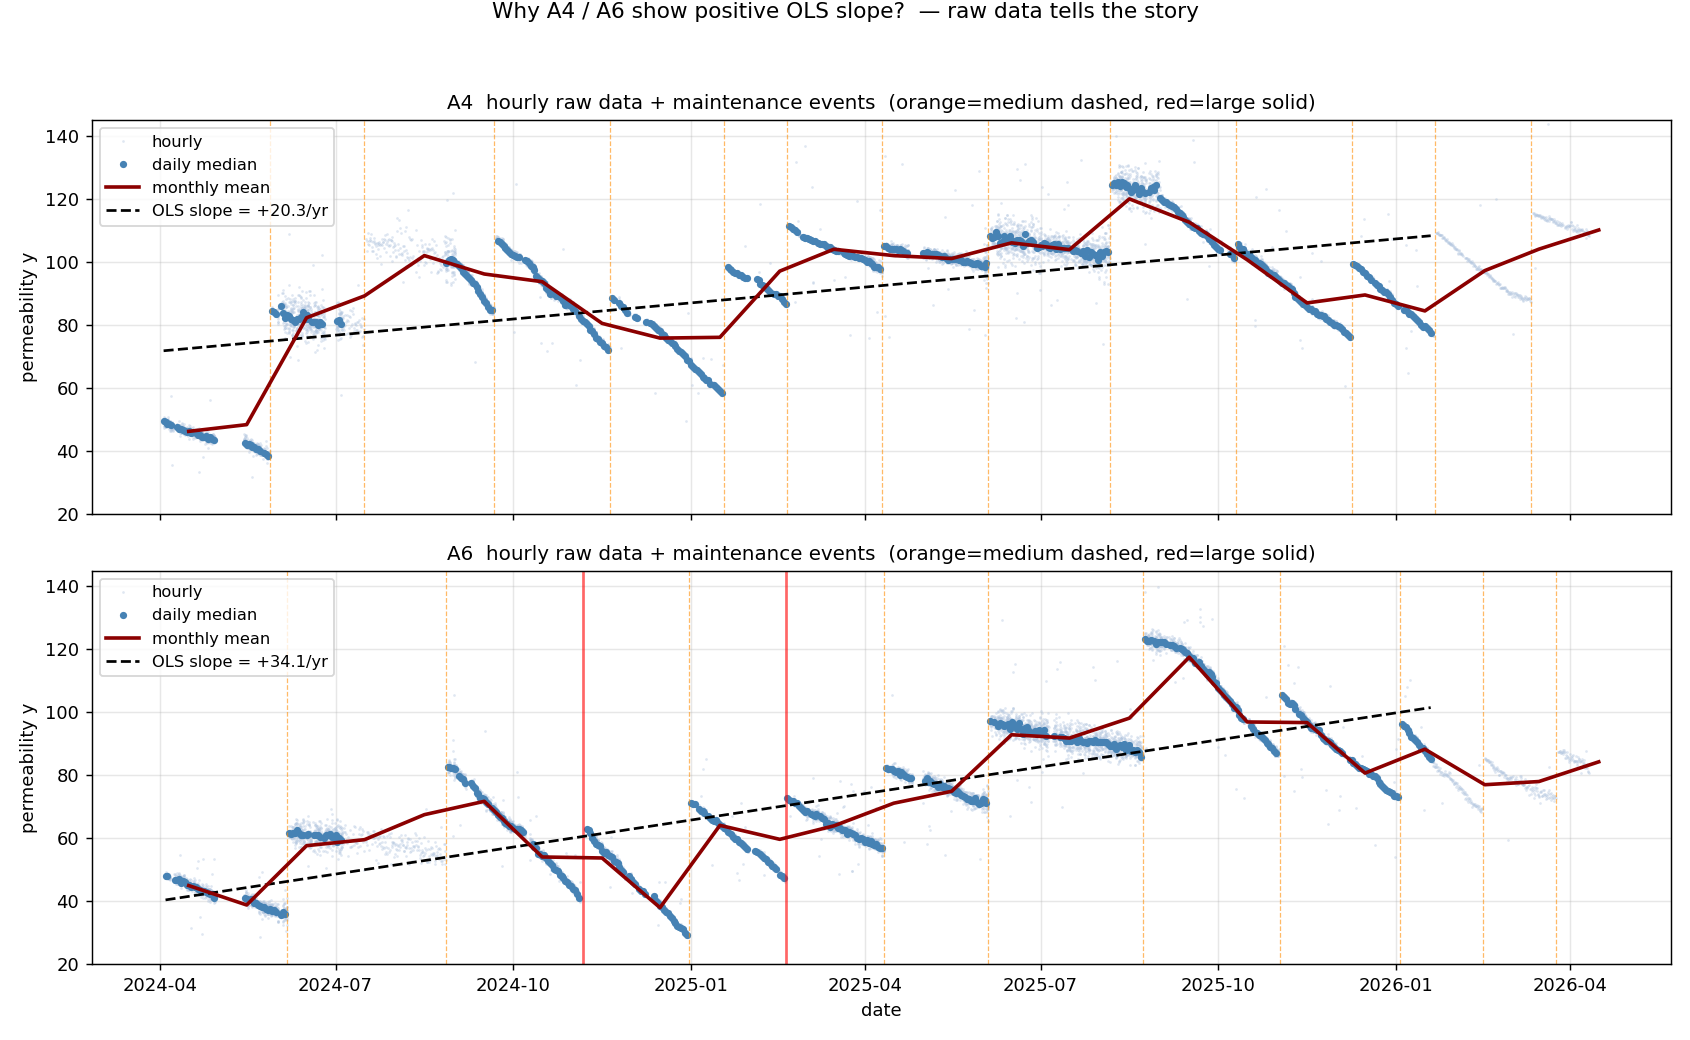
\includegraphics[width=0.95\textwidth]{diag_A4_A6_raw.png}
\caption{A4/A6 原始小时级数据 + 月均值 + OLS 拟合斜率。两台过滤器 2024-04 起始 y 值仅 46、45（其余 8 台均 $\ge 70$），暗示处于"启动期"未达稳态，OLS 把"基线爬升"误读为"自然衰减为正"。}
\label{fig:diagA4A6}
\end{figure}

% TODO: 插入图片对比表 + 季度均值轨迹

\subsection{Q1 主要图表}

\begin{figure}[H]
\centering
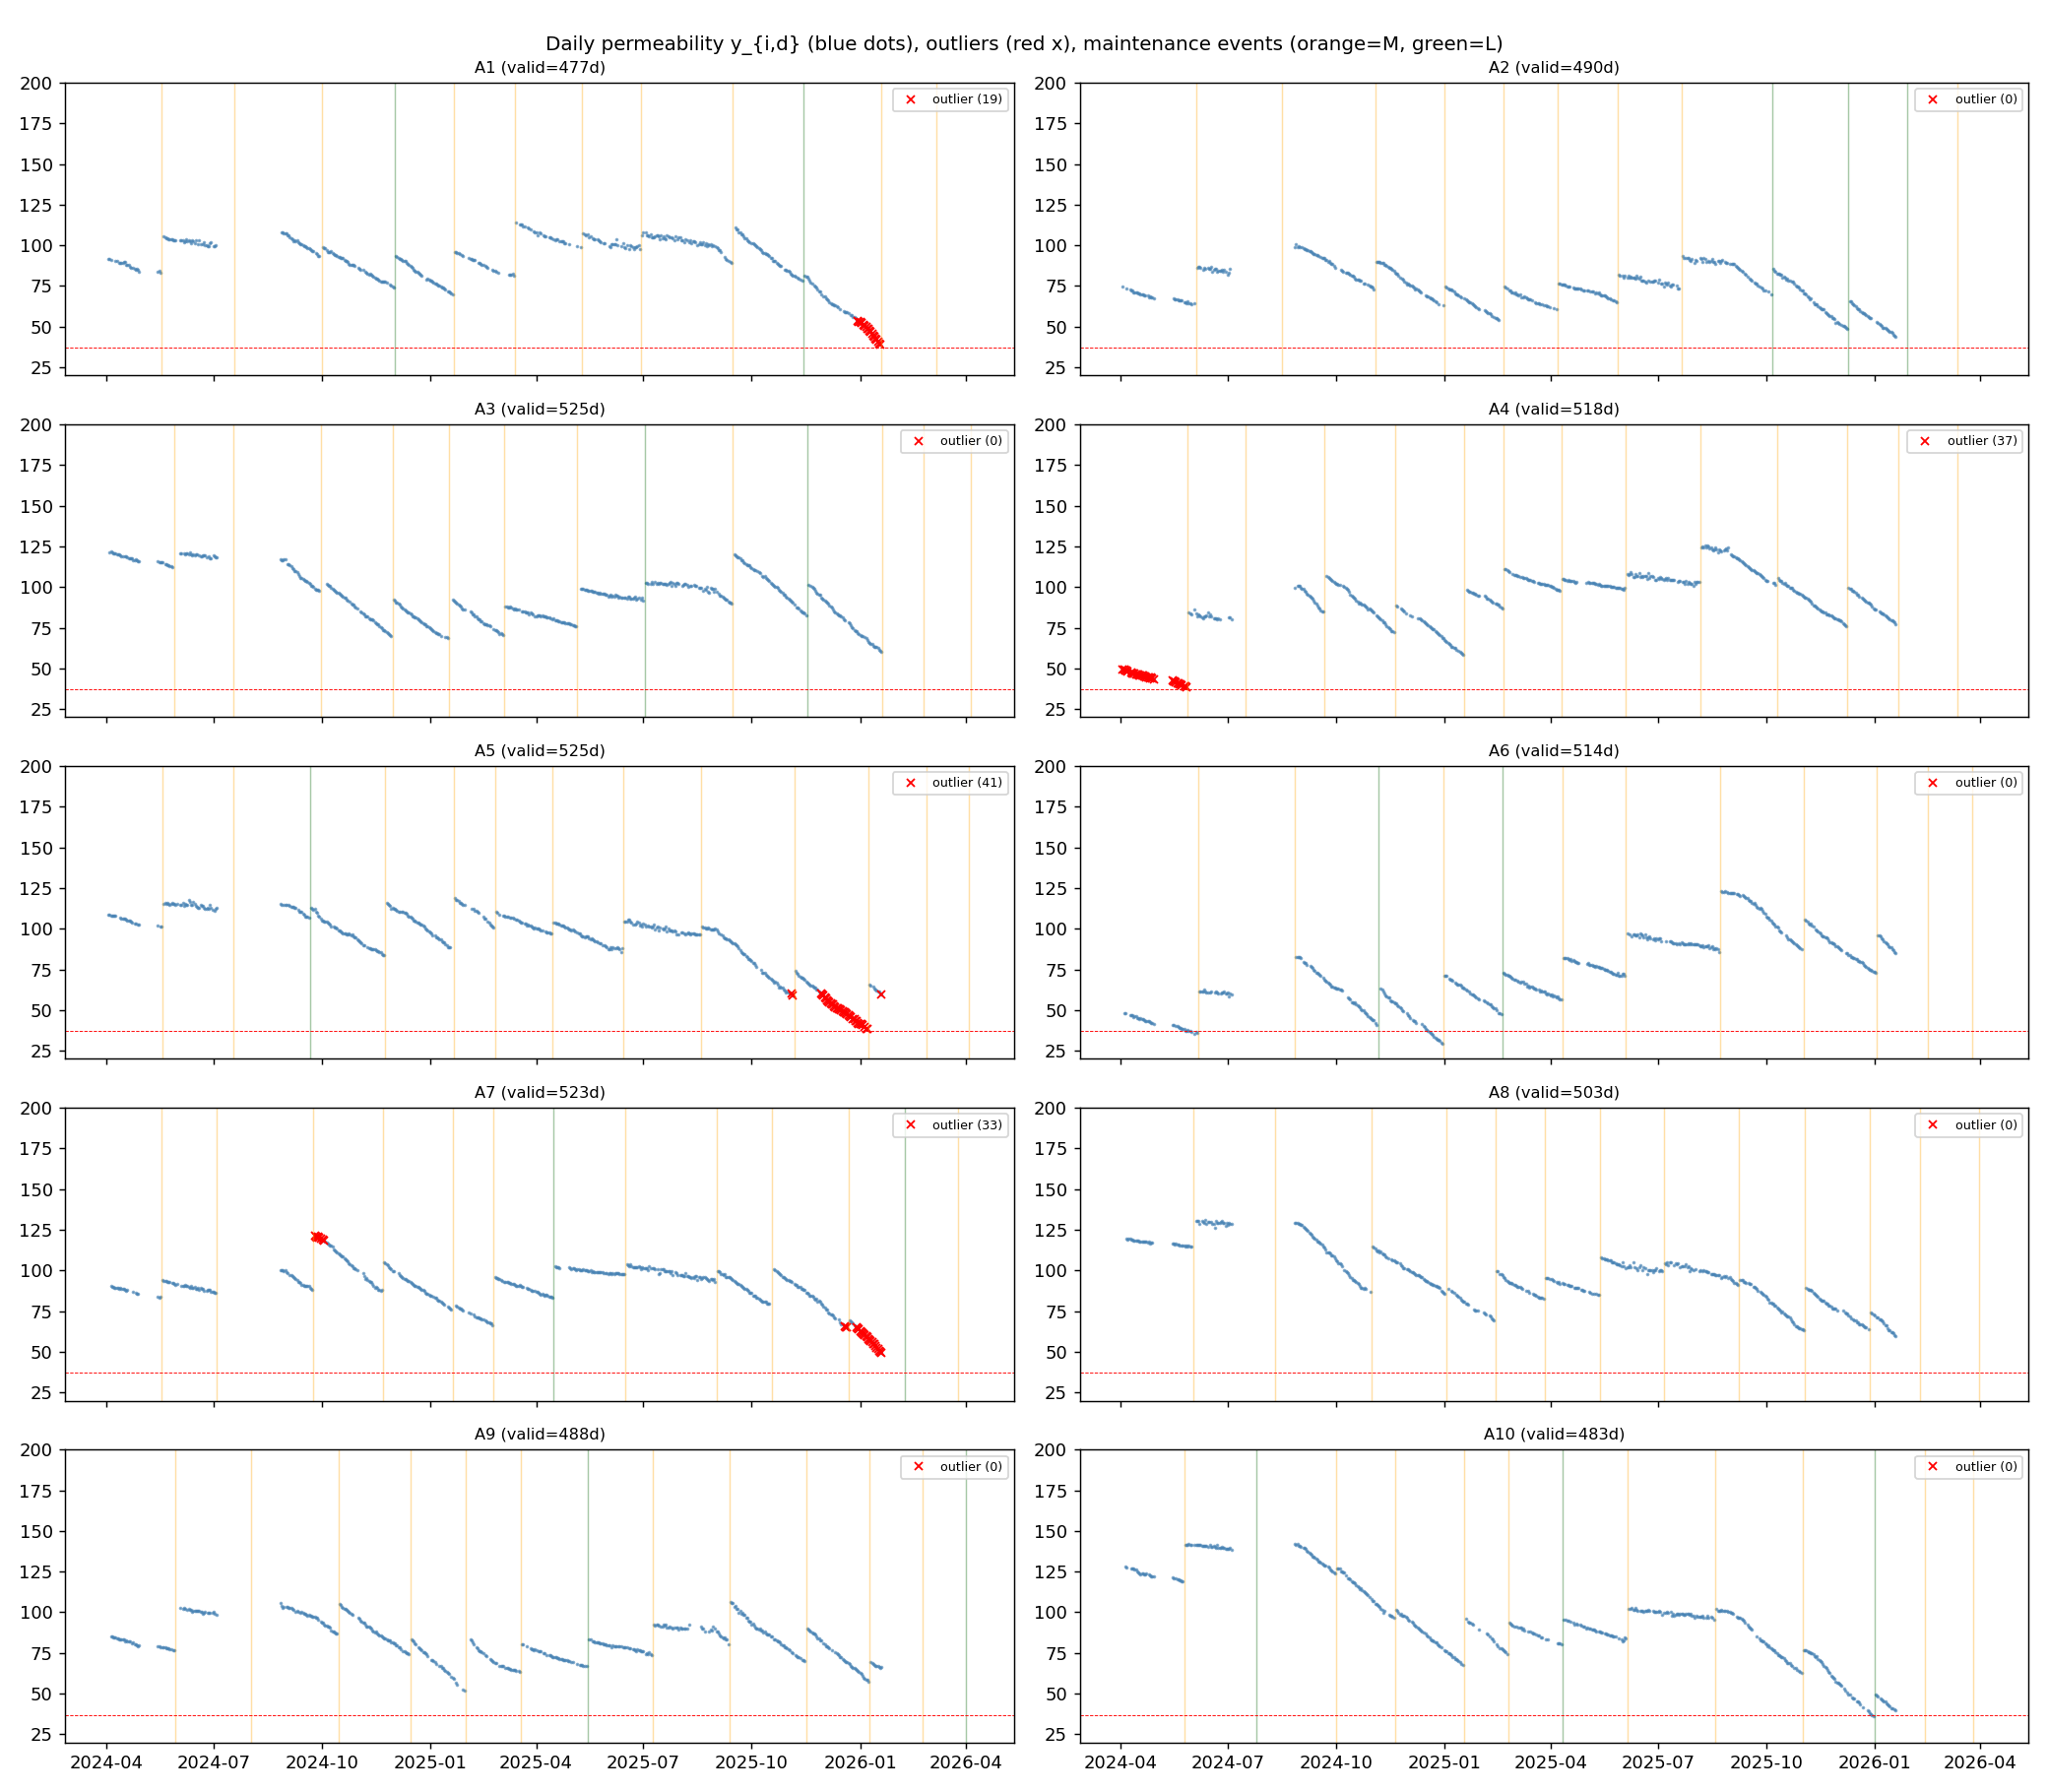
\includegraphics[width=\textwidth]{fig1_daily_series_outliers.png}
\caption{10 台过滤器日中位透水率 + 异常点 + 维护事件}
\label{fig:Q1_daily}
\end{figure}

\begin{figure}[H]
\centering
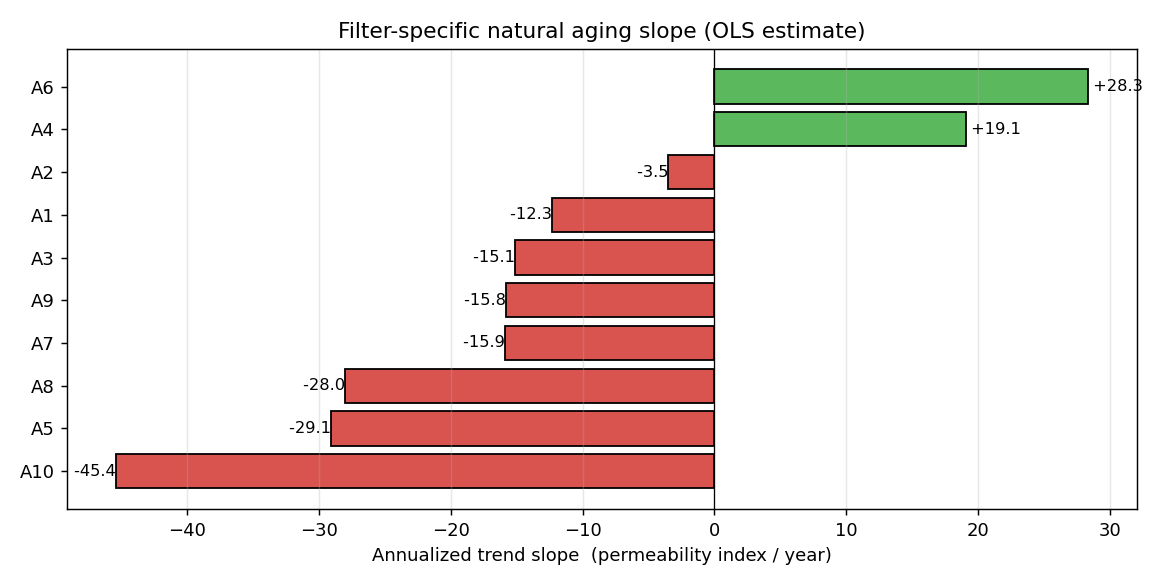
\includegraphics[width=0.85\textwidth]{fig4_trend_per_filter.png}
\caption{各过滤器自然衰减斜率 $\beta_i$（年化）}
\label{fig:Q1_beta}
\end{figure}

% =====================================================================
\section{Q2 模型建立与求解}

\subsection{当前固定维护规律}

从附件 2 抽取每台经验中位间隔作为 $(T_M^i, T_L^i)$。结果如下表（部分）：
% TODO: 插入 fixed_maintenance_rule.csv

A4、A8 两年内 0 次大维护，对应 $T_L^i = \infty$；A5 仅 1 次，回退为全样本中位 262.5 天。

\subsection{累积维护项的 CV 选参}

引入 $\gamma_m C_m + \gamma_l C_l$ 试图捕捉"维护越多衰减越快"，但 OLS 直接估计给出 $\hat{\gamma}_m = +9.9, \hat{\gamma}_l = +22.1$（与 $\beta_i \cdot t$ 共线导致符号错误）。在 $7 \times 7$ 网格上做时序 CV，最优 $(\gamma_m, \gamma_l) = (0.25, 2)$ 仅比 $\gamma = 0$ 改进 0.3\%，故采纳 $\gamma_m = \gamma_l = 0$（Occam 原则）。

\subsection{线性 vs 指数衰减比较}

\begin{table}[H]
\centering
\caption{线性 $y$ vs 指数 $\log y$ 拟合比较}
\begin{tabular}{lccc}
\toprule
模型 & 训练 RMSE & 验证 RMSE & 验证 MAE \\
\midrule
线性 $y$    & \textbf{7.41} & \textbf{12.96} & \textbf{10.14} \\
指数 $\log y$ & 7.93 & 13.59 & 10.23 \\
\bottomrule
\end{tabular}
\end{table}

线性模型胜出，作为 Q2.4 的前瞻仿真基石。

\subsection{向前 10 年仿真与寿命判定}

寿命定义：
\[
L_i = \min\{d \mid \bar{y}_i(d) < 37\}, \quad \bar{y}_i(d) = \frac{1}{365}\sum_{s=d-364}^{d} y_{i,s}
\]

\subsection{10 台寿命预测结果}

\begin{table}[H]
\centering
\caption{Q2 寿命预测（10 年地平线）}
\begin{tabular}{cccccc}
\toprule
$i$ & $L$（年） & 退役日期 & 起始年均值 & 跌破阈值年均值 & 状态 \\
\midrule
A10 & \textbf{1.15} & 2027-03 & 81.5 & 36.9 & 最先退役 \\
A8  & \textbf{1.89} & 2027-12 & 87.3 & 37.0 & 退役 \\
A9  & \textbf{2.68} & 2028-09 & 78.6 & 37.0 & 退役 \\
A3  & \textbf{3.26} & 2029-04 & 90.6 & 37.0 & 退役 \\
A5  & \textbf{6.35} & 2032-05 & 86.7 & 37.0 & 退役 \\
A1, A2, A7 & $> 10$ & --- & --- & --- & 维护有效 \\
A4, A6 & $> 10$ & --- & --- & --- & 模型外推不可靠 \\
\bottomrule
\end{tabular}
\end{table}

\begin{figure}[H]
\centering
\begin{subfigure}{0.45\textwidth}
  
\includegraphics[width=\linewidth]{fig_q2_life_bar.png}
  \caption{10 台预测寿命条形图}
\end{subfigure}
\hfill
\begin{subfigure}{0.45\textwidth}
  
\includegraphics[width=\linewidth]{fig_q2_rolling_avg.png}
  \caption{滚动 365 日均值与阈值 37}
\end{subfigure}
\caption{Q2 寿命预测可视化}
\end{figure}

% =====================================================================
\section{Q3 模型建立与求解}

\subsection{优化目标：等值年化成本（EAC）}

\begin{equation}
\boxed{\mathrm{EAC}_i(T_M, T_L) = \frac{c_{\text{buy}} + N_M(T_M, L) \cdot c_m + N_L(T_L, L) \cdot c_l}{L_i(T_M, T_L)}}
\label{eq:EAC}
\end{equation}

其中 $L_i$ 单位为年，寿命内维护总次数为：
\begin{align}
N_M(T_M, L) &= \frac{L \cdot 365.25}{T_M}, \\
N_L(T_L, L) &= \begin{cases} L \cdot 365.25 / T_L, & T_L < \infty \\ 0, & T_L = \infty \end{cases}.
\end{align}

每年频次记为 $n_M = N_M / L = 365.25 / T_M$，$n_L = N_L / L$，用于约束验证。

\subsection{决策变量与约束}

\begin{align}
\min_{T_M, T_L} \quad & \mathrm{EAC}_i(T_M, T_L) \\
\text{s.t.} \quad & 30 \le T_M \le 120 \quad\text{(每年 3.0--12.2 次中维护)} \\
& T_L \ge 91.3 \text{ 或 } T_L = \infty \quad\text{(每年 } 0 \le n_l \le 4 \text{ 次大维护)}
\end{align}

\subsection{求解方法：网格搜索}

$T_M \in \{30, 40, 50, 60, 70, 80, 90, 100, 120\}$（9 档），$T_L \in \{120, 180, 240, 300, 360, 450, 540, 720, \infty\}$（9 档），每台 81 组合 $\times$ 10 台 = 810 次 20 年地平线仿真，总耗时约 3.5 秒。

\subsection{10 台最优维护方案}

\begin{table}[H]
\centering
\caption{Q3 每台最优维护方案与 EAC}
\begin{tabular}{cccccccc}
\toprule
$i$ & $T_M^*$ (d) & $T_L^*$ (d) & $L^*$（年） & 退役 & $n_M$/年 & $n_L$/年 & EAC* (万/年) \\
\midrule
1  & 120 & 720 & 20.00$^*$ & 否 & 3.04 & 0.51 & 30.22 \\
2  & 80  & 450 & 8.47 & 是 & 4.57 & 0.81 & 58.88 \\
3  & 80  & 240 & 2.97 & 是 & 4.57 & 1.52 & 133.14 \\
4$^\dagger$  & 120 & $\infty$ & 20.00$^*$ & 否 & 3.04 & 0.00 & 24.13 \\
5  & 90  & 540 & 5.62 & 是 & 4.06 & 0.68 & 73.72 \\
6$^\dagger$  & 120 & $\infty$ & 20.00$^*$ & 否 & 3.04 & 0.00 & 24.13 \\
7  & 120 & 450 & 8.47 & 是 & 3.04 & 0.81 & 54.30 \\
8  & 60  & $\infty$ & 1.87 & 是 & 6.09 & 0.00 & 178.93 \\
9  & 60  & 300 & 2.87 & 是 & 6.09 & 1.22 & 137.33 \\
10 & 40  & 180 & 1.30 & 是 & 9.13 & 2.03 & 281.94 \\
\bottomrule
\end{tabular}
\\[0.5em]
\footnotesize $^*$ 20 年地平线截断，EAC 为上限。\quad $^\dagger$ A4/A6 模型外推不可靠，建议沿用历史经验维护。
\end{table}

\subsection{当前规律 vs 最优规律对比}

\textbf{合计节省 176.4 万元/年（15.0\%）}。详见图~\ref{fig:Q3_comp}。

\begin{figure}[H]
\centering
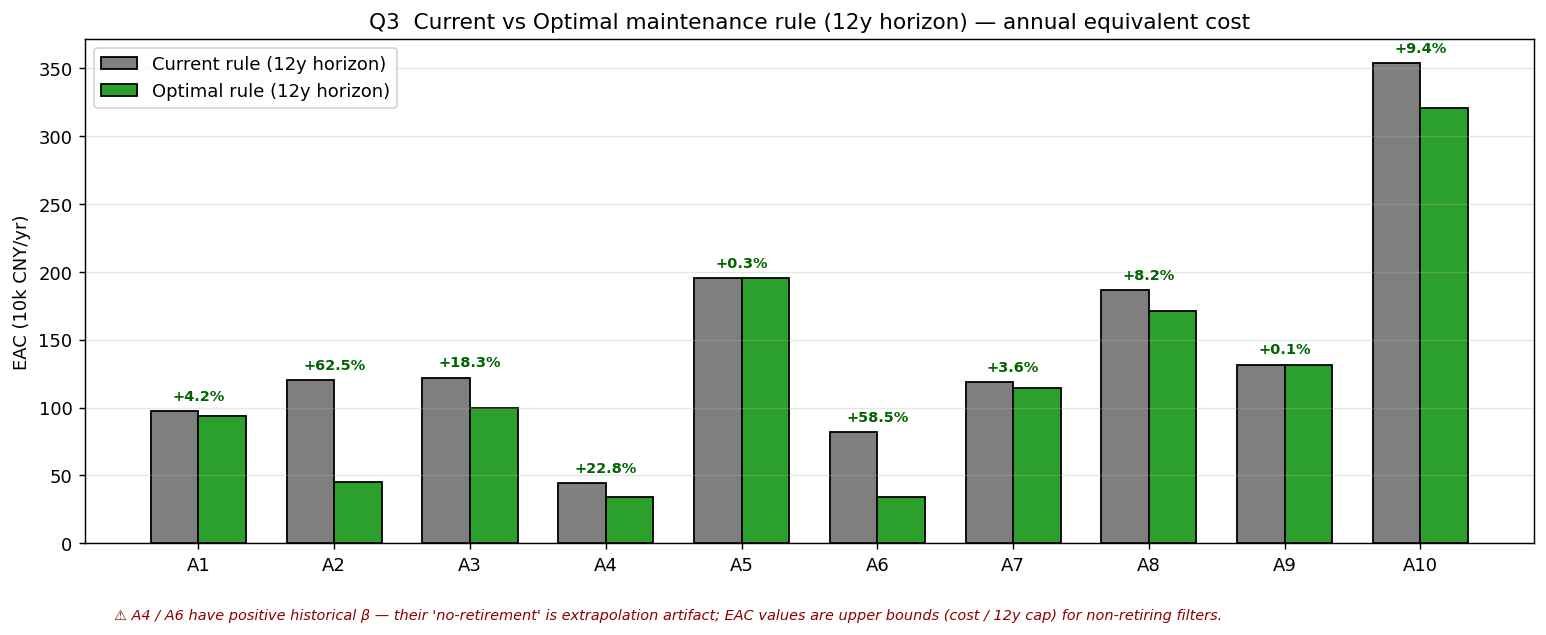
\includegraphics[width=\textwidth]{fig_q3_eac_comparison.png}
\caption{Q3 当前 vs 最优 EAC 对比（绿色百分比为节省比例）}
\label{fig:Q3_comp}
\end{figure}

\begin{figure}[H]
\centering
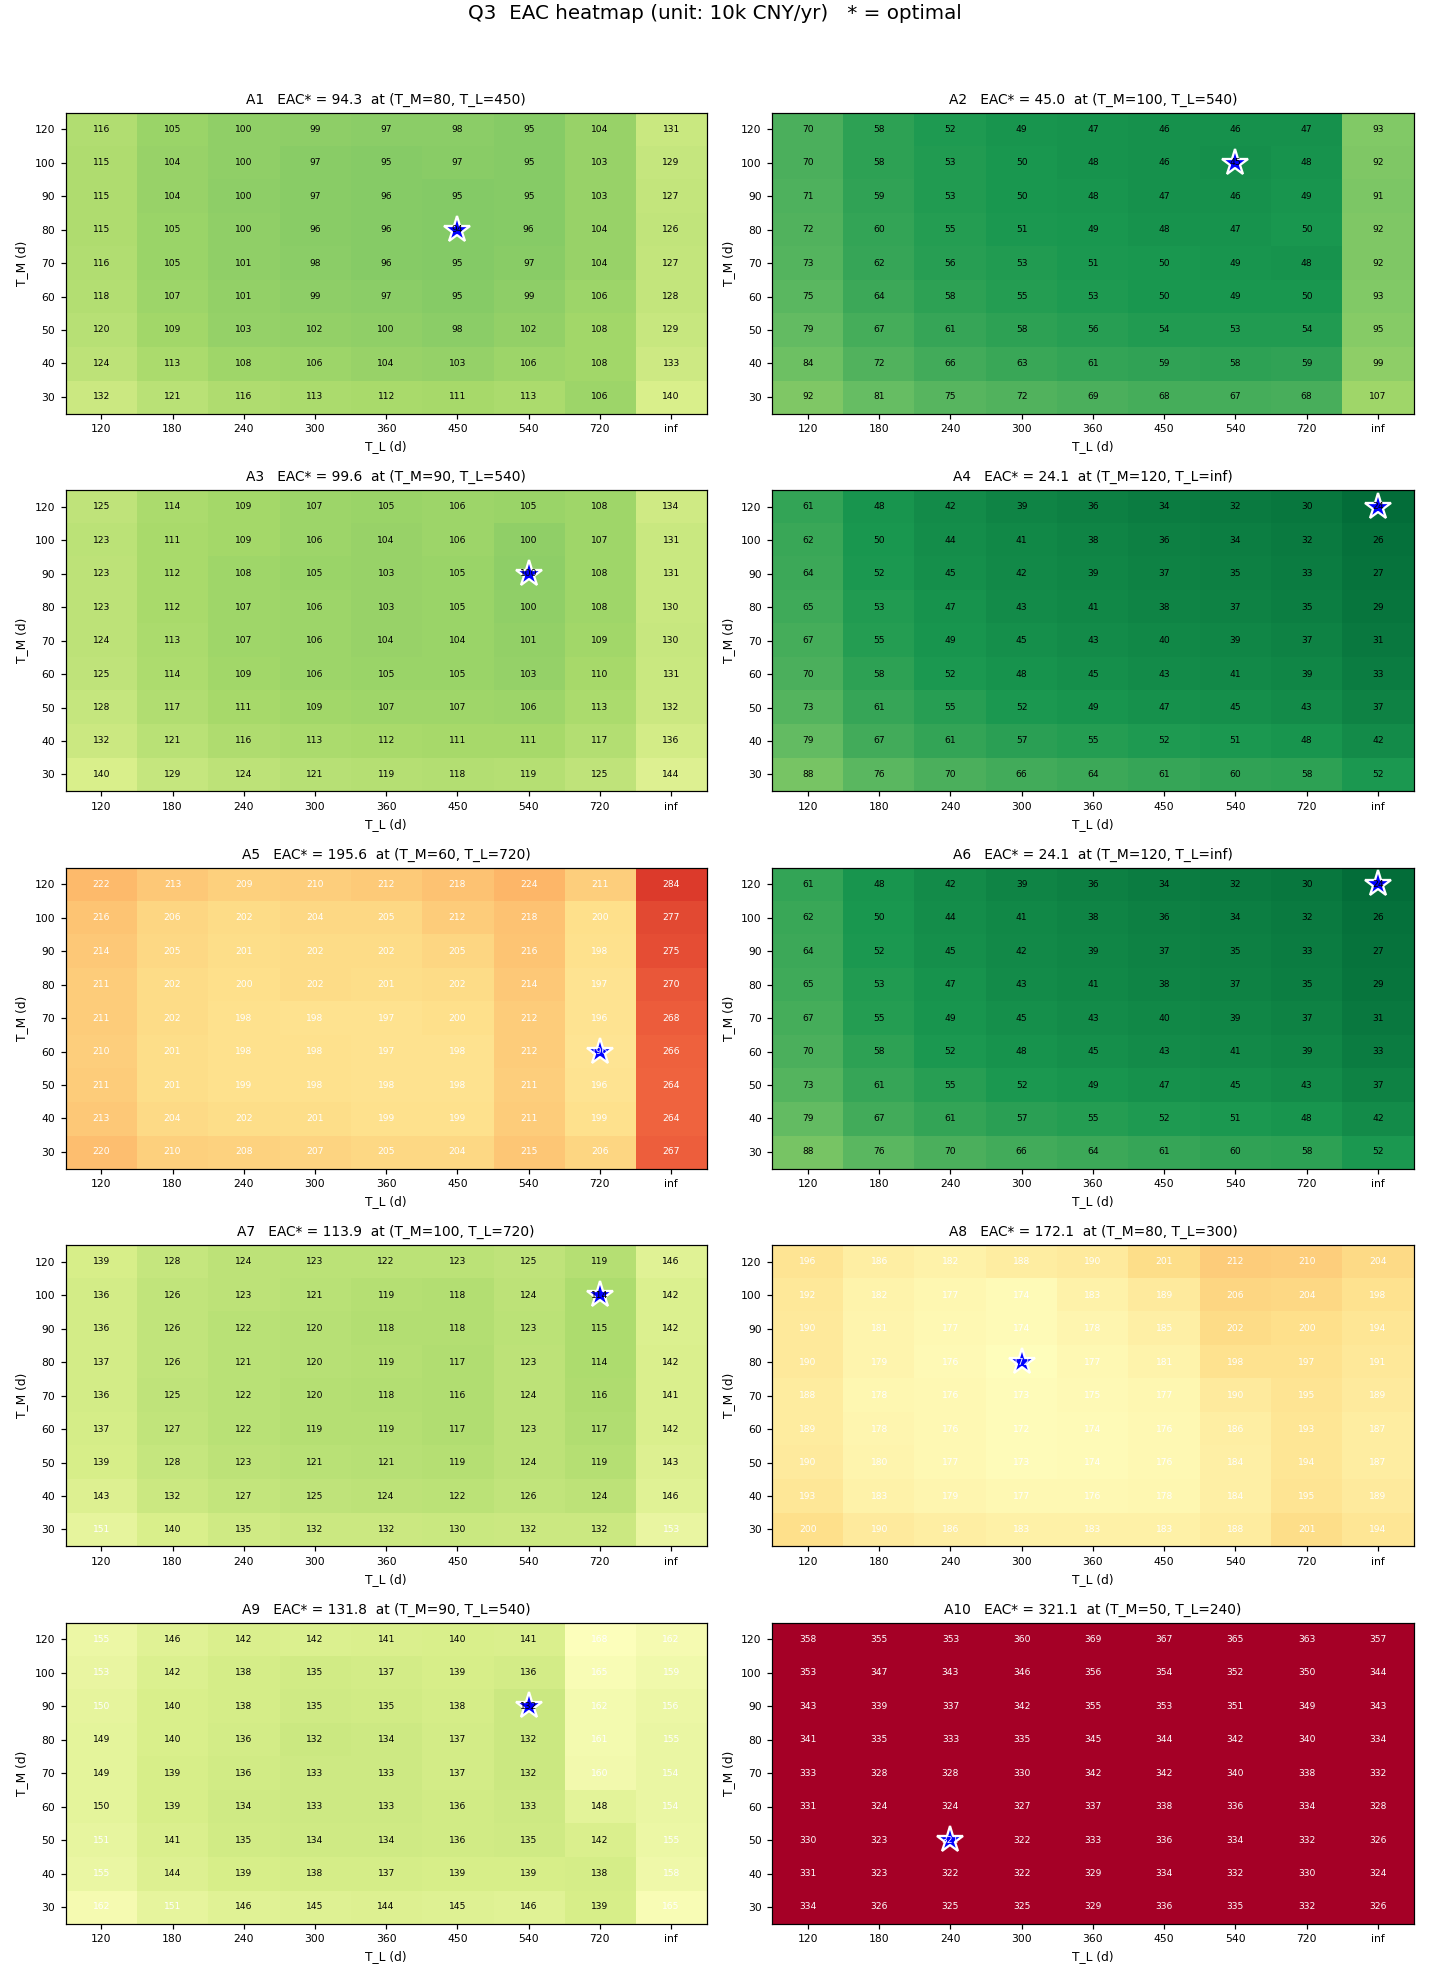
\includegraphics[width=0.95\textwidth]{fig_q3_eac_heatmap.png}
\caption{每台过滤器 EAC 关于 $(T_M, T_L)$ 的网格热力图（蓝星标记最优）}
\label{fig:Q3_heatmap}
\end{figure}

% =====================================================================
\section{Q4 模型建立与求解}

\subsection{敏感性分析设计}

对成本参数 $c_{\text{buy}}, c_m, c_l$ 在 $\{-30, -20, -10, 0, +10, +20, +30\}\%$ 七档扰动。

\subsection{加速计算}

观察到寿命 $L$、维护次数 $n_M, n_L$ 仅依赖 $(i, T_M, T_L)$ 与维护历史，\textbf{与成本参数无关}。因此 Q4 不需重跑 810 次仿真，只需在 Q3 已存的 \texttt{eac\_grid\_all.csv} 上重算 EAC：
\[
\mathrm{EAC}_i^{(c_{\text{buy}}', c_m', c_l')} = \frac{c_{\text{buy}}' + n_M c_m' + n_L c_l'}{L}
\]
将 $7^3 \times 810 = 277{,}830$ 次仿真压缩到 $7^3 = 343$ 次表查询。

\subsection{弹性分析}

定义弹性 $\varepsilon = \frac{\Delta \mathrm{EAC} / \mathrm{EAC}}{\Delta c / c}$。全队层面：

\begin{table}[H]
\centering
\caption{全队 EAC 关于成本参数的弹性}
\begin{tabular}{lcccc}
\toprule
参数 & 弹性 $\varepsilon$ & $-30\%$ EAC & 基准 EAC & $+30\%$ EAC \\
\midrule
$c_{\text{buy}}$ & \textbf{0.764} & 764.21 & 996.76 & 1223.08 \\
$c_m$            & 0.141 & 953.83 & 996.76 & 1036.49 \\
$c_l$            & 0.094 & 965.07 & 996.76 & 1023.98 \\
\bottomrule
\end{tabular}
\end{table}

\begin{figure}[H]
\centering
\begin{subfigure}{0.49\textwidth}
  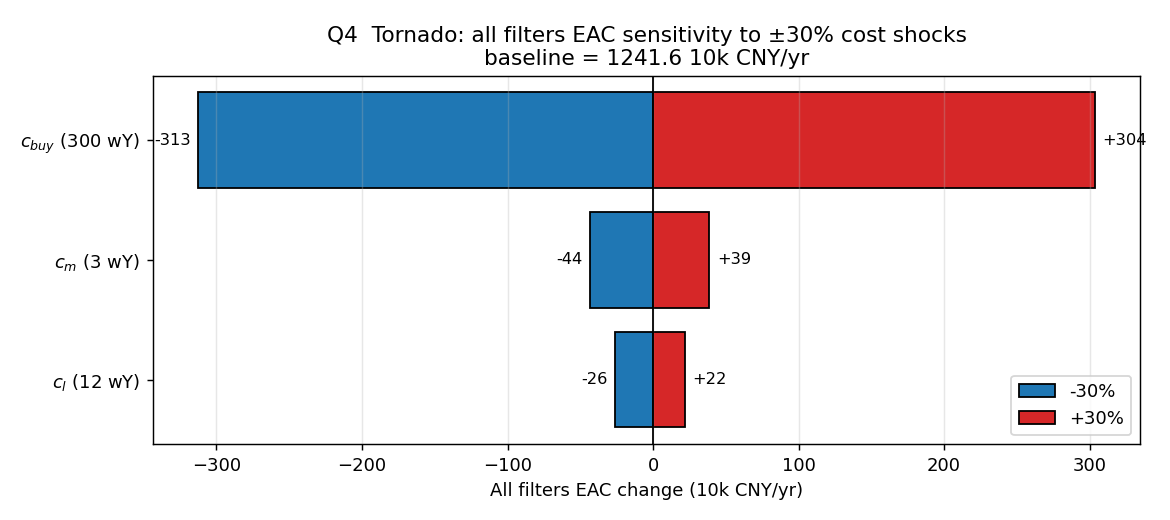
\includegraphics[width=\linewidth]{fig_q4_tornado.png}
  \caption{龙卷风图：全队 EAC 对 $\pm 30\%$ 成本的响应}
\end{subfigure}
\hfill
\begin{subfigure}{0.49\textwidth}
  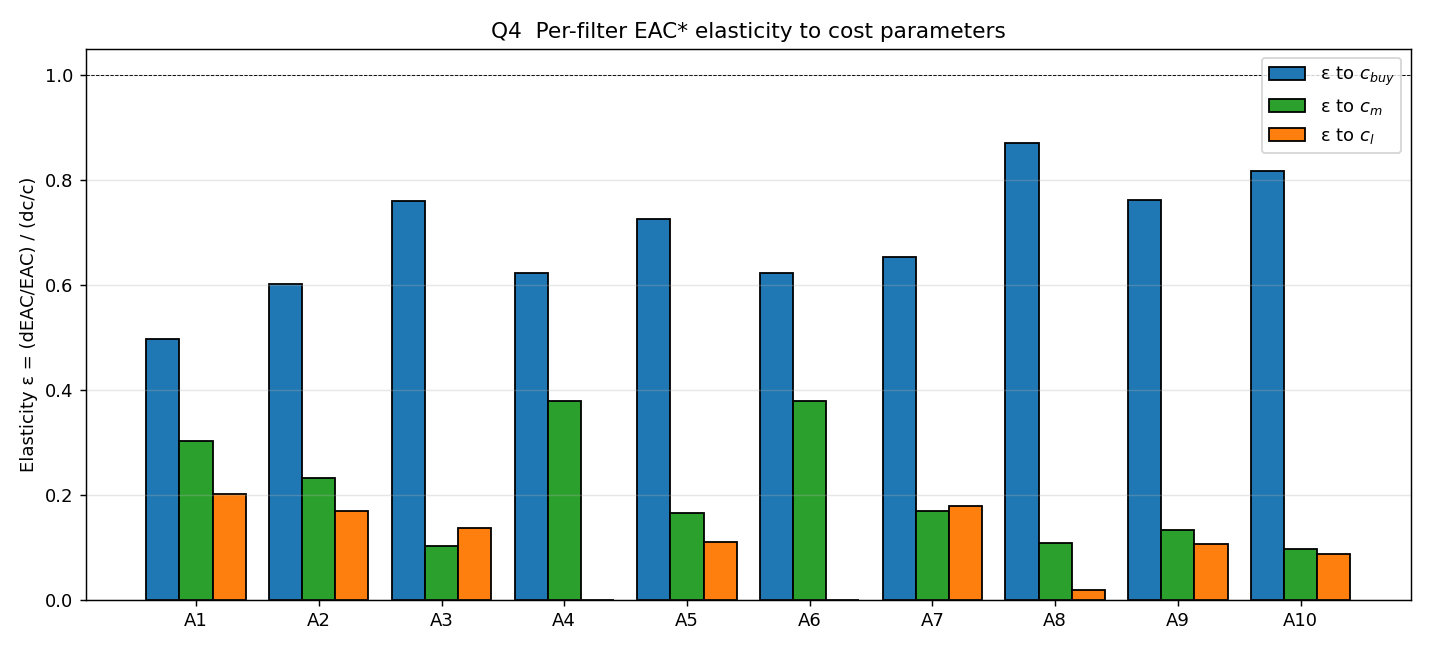
\includegraphics[width=\linewidth]{fig_q4_elasticity.png}
  \caption{每台 EAC* 弹性分解}
\end{subfigure}
\caption{Q4 敏感性可视化}
\end{figure}

\subsection{方案稳健性}

\begin{itemize}[leftmargin=2em]
  \item \textbf{完全稳定（5 台）}：A1, A4, A5, A6, A7 在 21 个单参数场景下方案不变；
  \item \textbf{边界切换（3 台）}：A2, A3, A9 仅在 $\pm 30\%$ 极值处切换；
  \item \textbf{较敏感（2 台）}：A8, A10 寿命短，对 $c_{\text{buy}}$ 弹性达 0.82--0.87，建议动态调整。
\end{itemize}

\subsection{联合敏感性与极端场景}

\begin{table}[H]
\centering
\caption{三参数同向 $\pm 30\%$ 极端场景}
\begin{tabular}{lcc}
\toprule
场景 & 全队 EAC（万元/年） & 偏离基准 \\
\midrule
全部 $-30\%$（最好） & 697.7 & $-30.0\%$ \\
基准 & 996.8 & --- \\
全部 $+30\%$（最坏） & 1295.8 & $+30.0\%$ \\
\bottomrule
\end{tabular}
\end{table}

\begin{figure}[H]
\centering

\includegraphics[width=0.85\textwidth]{fig_q4_joint_heatmap.png}
\caption{$c_{\text{buy}} \times c_l$ 联合扰动下的全队 EAC 总和}
\end{figure}

% =====================================================================
\section{模型评价与改进}

\subsection{优点}
\begin{itemize}[leftmargin=2em]
  \item 模型层次清晰，Q1 $\to$ Q2 $\to$ Q3 $\to$ Q4 数值逐级一致（已核查）；
  \item 用网格 CV 解决了累积维护项的共线性陷阱；
  \item EAC 公式利用维护频次与成本无关的解耦特性，大幅加速 Q4；
  \item 对 A4/A6 异常进行追溯诊断，明确数据特征是"启动期"而非建模 bug。
\end{itemize}

\subsection{缺点}
\begin{itemize}[leftmargin=2em]
  \item 线性时间趋势对 A4/A6 启动期不适用，Q2-Q4 报告中已警示但未独立建模；
  \item 网格搜索步长 10 天，可能存在 1-3\% 的离散化噪声（A8 / A10 表现明显）；
  \item 滚动 365 日均值在外推前 365 天混合观测与模拟值，存在轻微失真。
\end{itemize}

\subsection{改进方向}
\begin{itemize}[leftmargin=2em]
  \item 对 A4/A6 引入 "启动期" 哑变量分段拟合；
  \item 用梯度法或贝叶斯优化替代网格搜索；
  \item 引入维护质量随机性（$\delta_m, \delta_l$ 服从分布而非确定值），跑蒙特卡洛得寿命置信区间。
\end{itemize}

% =====================================================================
\begin{thebibliography}{9}
  \bibitem{ols} Greene W.H. \emph{Econometric Analysis}, 8th ed., Pearson, 2018.
  \bibitem{stl} Cleveland R.B., et al. STL: A seasonal-trend decomposition procedure based on Loess. \emph{J. Off. Stat.} 6(1):3-73, 1990.
  \bibitem{eac} Park C.S. \emph{Contemporary Engineering Economics}, 6th ed., Pearson, 2016.
\end{thebibliography}

% =====================================================================
\appendix

\section{Q1 OLS 系数完整列表}
% TODO: 插入 reg_summary_full.csv 完整 28 行

\section{核心代码片段}

\subsection{Q1 主回归}
\begin{lstlisting}[caption={Q1 step6\_ols\_wls.py 主体}]
# 设计矩阵：const + I(i=2..10) + t_i*1..10 + sin1 + cos1
#         + H_m7 + H_l7 + A_m_f + A_l_f + has_m + has_l (28 列)
X, names = build_X(df, add_filter_specific_trend=True)
beta, *_ = np.linalg.lstsq(X, df["y"].values, rcond=None)
yhat = X @ beta
r2 = 1 - ((y - yhat)**2).sum() / ((y - y.mean())**2).sum()
\end{lstlisting}

\subsection{Q3 网格搜索}
\begin{lstlisting}[caption={Q3 step1\_grid\_search\_eac.py 主循环}]
for i in range(1, 11):
    best = dict(EAC=np.inf)
    for T_M in T_M_grid:
        for T_L in T_L_grid:
            y_sim = simulate_y(i, T_M, T_L)
            L = compute_life_days(i, y_sim) / 365.25
            n_M = L * 365.25 / T_M
            n_L = L * 365.25 / T_L if np.isfinite(T_L) else 0.0
            EAC = (C_BUY + n_M*C_M + n_L*C_L) / L
            if EAC < best["EAC"]:
                best = dict(T_M=T_M, T_L=T_L, L=L, EAC=EAC)
\end{lstlisting}

\subsection{Q4 加速重计算}
\begin{lstlisting}[caption={Q4 step1\_single\_param\_sweep.py 加速}]
def best_per_filter(c_buy, c_m, c_l):
    g = grid.copy()
    g["EAC_new"] = (c_buy + g["n_M"]*c_m + g["n_L"]*c_l) / g["L_years"]
    return g.loc[g.groupby("i")["EAC_new"].idxmin()]
\end{lstlisting}

\section{完整数据文件清单}

\begin{itemize}[leftmargin=2em]
  \item \texttt{Q1输出/}：9 个 step 脚本 + 5 个 CSV + 5 张图 + Q1\_summary.md
  \item \texttt{Q2输出/}：7 个 step 脚本 + 8 个 CSV + 3 张图 + Q2\_summary.md
  \item \texttt{Q3输出/}：5 个 step 脚本 + 5 个 CSV + 3 张图 + Q3\_summary.md
  \item \texttt{Q4输出/}：4 个 step 脚本 + 6 个 CSV + 4 张图 + Q4\_summary.md
\end{itemize}

\end{document}
